
\bta{练习使用多用表}



\begin{enumerate}
%\renewcommand{\labelenumi}{\arabic{enumi}.}
% A(\Alph) a(\alph) I(\Roman) i(\roman) 1(\arabic)
%设定全局标号series=example	%引用全局变量resume=example
%[topsep=-0.3em,parsep=-0.3em,itemsep=-0.3em,partopsep=-0.3em]
%可使用leftmargin调整列表环境左边的空白长度 [leftmargin=0em]
\item
\exwhere{$ 2019 $ 年物理全国\lmd{3}卷}
某同学欲将内阻为 $ 98.5 \ \Omega $、量程为 $ 100 \ uA $ 的电流表改装成欧姆表并进行刻
度和校准,要求改装后欧姆表的 $ 15 \ k\Omega $刻度正好对应电流表表盘的 $ 50 \ uA $ 刻度。可选用的器材还有:
定值电阻 $ R_{0} $(阻值 $ 14 \ k\Omega $),滑动变阻器 $ R_{1} $(最大阻值 $ 1500 \ \Omega $),滑动变阻器 $ R_{2} $(最大阻值 $ 500 \ \Omega $),
电阻箱($ 0 \sim 99999.9 \ \Omega $),干电池($ E=1.5 \ V $,$ r=1.5 \ \Omega $),红、黑表笔和导线若干。
\begin{figure}[h!]
\centering
\begin{subfigure}{0.4\linewidth}
\centering
\includesvg[width=0.7\linewidth]{picture/svg/GZ-3-tiyou-0990} 
\caption{}\label{}
\end{subfigure}
\begin{subfigure}{0.4\linewidth}
\centering
\includesvg[width=0.7\linewidth]{picture/svg/GZ-3-tiyou-0991} 
\caption{}\label{}
\end{subfigure}
\begin{subfigure}{0.4\linewidth}
\centering
\includesvg[width=0.7\linewidth]{picture/svg/GZ-3-tiyou-0992} 
\caption{}\label{}
\end{subfigure}
\end{figure}


\begin{enumerate}
%\renewcommand{\labelenumi}{\arabic{enumi}.}
% A(\Alph) a(\alph) I(\Roman) i(\roman) 1(\arabic)
%设定全局标号series=example	%引用全局变量resume=example
%[topsep=-0.3em,parsep=-0.3em,itemsep=-0.3em,partopsep=-0.3em]
%可使用leftmargin调整列表环境左边的空白长度 [leftmargin=0em]
\item
欧姆表设计

将图($ a $)中的实物连线组成欧姆表。
欧姆表改装好后,滑动变阻器 $ R $ 接入电路的电
阻应为 \underlinegap $ \Omega $:滑动变阻器选 \underlinegap (填“$ R_{1} $”或“$ R_{2} $”)。



\item 
刻度欧姆表表盘

通过计算,对整个表盘进行电阻刻度,如图($ b $)所示。表盘上 $ a $、$ b $ 处的电流刻度分别为 $ 25 $ 和 $ 75 $,
则 $ a $、$ b $ 处的电阻刻度分别为 \underlinegap 、 \underlinegap 。


\item 
校准

红、黑表笔短接,调节滑动变阻器,使欧姆表指针指向 \underlinegap $ k \Omega $处;将红、黑表笔与电阻箱连接,记
录多组电阻箱接入电路的电阻值及欧姆表上对应的测量值,完成校准数据测量。若校准某刻度时,
电阻箱旋钮位置如图($ c $)所示,则电阻箱接入的阻值为 \underlinegap $ \Omega $。




\end{enumerate}


\tk{
\begin{enumerate}
%\renewcommand{\labelenumi}{\arabic{enumi}.}
% A(\Alph) a(\alph) I(\Roman) i(\roman) 1(\arabic)
%设定全局标号series=example	%引用全局变量resume=example
%[topsep=-0.3em,parsep=-0.3em,itemsep=-0.3em,partopsep=-0.3em]
%可使用leftmargin调整列表环境左边的空白长度 [leftmargin=0em]
\item
$ 900 $ \quad $ R_{1} $
连线如图:
\begin{center}
\includesvg[width=0.23\linewidth]{picture/svg/GZ-3-tiyou-0993} 	
\end{center}
\item 	
$ 45 $ \quad $ 5 $
\item 	
$ 0 $ \quad $ 35000.0 $
\end{enumerate}
} 

\item 
\exwhere{$ 2011 $ 年理综北京卷}
用如图 $ 1 $ 所示的多用电表测量电阻,要用到选择开关 $ K $ 和两个部件 $ S $、$ T $。请根据下列步骤完成电
阻测量:

①旋动部件 \underlinegap ,使指针对准电流的“$ 0 $”刻线。

②将 $ K $ 旋转到电阻挡“$ \times 10^{0} $”的位置。



③将插入“$ + $”、“$ - $”插孔的表笔短接,旋动部件 \underlinegap ,使指针对准
电阻的 \underlinegap (填“$ 0 $ 刻线”或“$ \infty $刻线”。


④将两表笔分别与待测电阻相接,发现指针偏转角度过小。为了得
到比较准确的测量结果,请从下列选项中挑出合理的步骤,并按 \underlinegap 
的顺序进行操作,再完成读数测量。
\begin{figure}[h!]
\centering
\includesvg[width=0.23\linewidth]{picture/svg/GZ-3-tiyou-0994}
\end{figure}


\fourchoices
{将 $ K $ 旋转到电阻挡“$ \times 1k $”的位置}
{将 $ K $ 旋转到电阻挡“$ \times 10 $”的位置}
{将两表笔的金属部分分别与被测电阻的两根引线相接}
{将两表笔短接,旋动合适部件,对电表进行校准}







\item
\exwhere{$ 2011 $ 年理综重庆卷}
某电动机的三组线圈①、②、③阻值相同,均为几欧姆,接法可能是图 $ 1 $ 中甲、乙两种之
一,$ A $、$ B $ 和 $ C $ 是外接头。现有一组线圈断路,维修人员通
过多用电表测量外接头之间的电阻来判断故障,若测量 $ A $
和 $ B $ 之间、$ B $ 和 $ C $ 之间、$ A $ 和 $ C $ 之间的电阻时,多用电表
指针偏转分别如图 $ 2(a) $、$ (b) $、$ (c) $所示,则测量中使用的欧
姆档的倍率是 \underlinegap (填 $ \times 1 $、 $ \times 10 $、 $ \times 100 $ 或 $ \times 1k $ ),三组线圈的接法是 \underlinegap (填甲或乙),断路线圈是 \underlinegap (填①、②或③)。
\begin{figure}[h!]
\centering
\begin{subfigure}{0.4\linewidth}
\centering
\includesvg[width=0.7\linewidth]{picture/svg/GZ-3-tiyou-0995} 
\caption{}\label{}
\end{subfigure}
\begin{subfigure}{0.8\linewidth}
\centering
\includesvg[width=0.8\linewidth]{picture/svg/GZ-3-tiyou-0996} 
\caption{}\label{}
\end{subfigure}
\end{figure}


\tk{$ \times 1 $ \quad 乙 \quad ③} 


\item 
\exwhere{$ 2014 $ 年理综重庆卷}
某照明电路出现故障,其电路如图 $ 1 $ 所示,该电路用标称值 $ 12 \ V $ 的蓄电池为电源,导线及其接
触完好。维修人员使用已调好的多用表直流 $ 50 \ V $ 挡检测故障。他将黑表笔接在 $ c $ 点,用红表笔分别
探测电路的 $ a $、$ b $ 点。
\begin{figure}[h!]
\centering
\begin{subfigure}{0.4\linewidth}
\centering
\includesvg[width=0.7\linewidth]{picture/svg/GZ-3-tiyou-0997} 
\caption{}\label{}
\end{subfigure}
\begin{subfigure}{0.4\linewidth}
\centering
\includesvg[width=0.7\linewidth]{picture/svg/GZ-3-tiyou-0998} 
\caption{}\label{}
\end{subfigure}

\end{figure}

\begin{enumerate}
%\renewcommand{\labelenumi}{\arabic{enumi}.}
% A(\Alph) a(\alph) I(\Roman) i(\roman) 1(\arabic)
%设定全局标号series=example	%引用全局变量resume=example
%[topsep=-0.3em,parsep=-0.3em,itemsep=-0.3em,partopsep=-0.3em]
%可使用leftmargin调整列表环境左边的空白长度 [leftmargin=0em]
\item
断开开关,红表笔接 $ a $ 点时多用表指示如题图 $ 2 $ 所示,读数为 \underlinegap 
$ V $,说明 \underlinegap 
正常(选
填:蓄电池、保险丝、开关、小灯)。


\item 
红表笔接 $ b $ 点,断开开
关时,表针不偏转,闭合
开关后,多用表指示仍然
和题图 $ 2 $ 相同,可判断
发生故障的器件
是 \underlinegap 。(选填:蓄电池、保险丝、开关、小灯)


\end{enumerate}


\tk{
\begin{enumerate}
%\renewcommand{\labelenumi}{\arabic{enumi}.}
% A(\Alph) a(\alph) I(\Roman) i(\roman) 1(\arabic)
%设定全局标号series=example	%引用全局变量resume=example
%[topsep=-0.3em,parsep=-0.3em,itemsep=-0.3em,partopsep=-0.3em]
%可使用leftmargin调整列表环境左边的空白长度 [leftmargin=0em]
\item
$11.5 \quad(11.2 \sim 11.8)$;蓄电池
\item 
小灯
\end{enumerate}
} 

\item 
\exwhere{$ 2013 $ 年上海卷}
为确定某电子元件的电气特性,做如下测量。
\begin{figure}[h!]
\centering
\begin{subfigure}{0.4\linewidth}
\centering
\includesvg[width=0.7\linewidth]{picture/svg/GZ-3-tiyou-0999} 
\caption{}\label{}
\end{subfigure}
\begin{subfigure}{0.4\linewidth}
\centering
\includesvg[width=0.7\linewidth]{picture/svg/GZ-3-tiyou-1000} 
\caption{}\label{}
\end{subfigure}
\end{figure}

\begin{enumerate}
%\renewcommand{\labelenumi}{\arabic{enumi}.}
% A(\Alph) a(\alph) I(\Roman) i(\roman) 1(\arabic)
%设定全局标号series=example	%引用全局变量resume=example
%[topsep=-0.3em,parsep=-0.3em,itemsep=-0.3em,partopsep=-0.3em]
%可使用leftmargin调整列表环境左边的空白长度 [leftmargin=0em]
\item
用多用表测量该元件的电阻,选用“$ \times 100 $”倍率的电阻
档测量,发现多用表指针偏转过大,因此需选择 \underlinegap 0倍
率的电阻档(填:“$ \times 10 $”或“$ \times 1k $”),并 \underlinegap 再进行
测量,多用表的示数如图$ (a) $所示,测量结果
为 \underlinegap 
$ \Omega $。




\item 
将待测元件(额定电压 $ 9 \ V $)、蓄电池、滑动变阻器、
电流表、多用表、电键及若干导线连接成电路如图$ (b) $所
示。添加连线,使电路能测量该元件完整的伏安特性。



本实验中使用多用表测电压,多用表的选择开关应调到 \underlinegap 档(填:“直流电压 $ 10 \ V $”
或“直流电压 $ 50 \ V $”)。




\end{enumerate}

\tk{
\begin{enumerate}
%\renewcommand{\labelenumi}{\arabic{enumi}.}
% A(\Alph) a(\alph) I(\Roman) i(\roman) 1(\arabic)
%设定全局标号series=example	%引用全局变量resume=example
%[topsep=-0.3em,parsep=-0.3em,itemsep=-0.3em,partopsep=-0.3em]
%可使用leftmargin调整列表环境左边的空白长度 [leftmargin=0em]
\item
$ \times 10 $ \quad 欧姆调零 \quad $ 70 $
\item 
电路如图;直流电压 $ 10 \ V $ 档
\begin{center}
\includesvg[width=0.23\linewidth]{picture/svg/GZ-3-tiyou-1001} 
\end{center}
\end{enumerate}
} 

\item 
\exwhere{$ 2013 $ 年新课标 \lmd{1} 卷}
某学生实验小组利用图$ (a) $所示电路,测量多用电表内电池的电动势和电阻“$ \times 1k $”挡内部
电路的总电阻。使用的器材有:\\
多用电表;\\
电压表:量程 $ 5 \ V $,内阻十几千欧;\\
滑动变阻器:最大阻值 $ 5 \ k\Omega $;\\
导线若干。

回答下列问题:
\begin{figure}[h!]
\centering
\begin{subfigure}{0.4\linewidth}
\centering
\includesvg[width=0.7\linewidth]{picture/svg/GZ-3-tiyou-1002} 
\caption{}\label{}
\end{subfigure}
\begin{subfigure}{0.4\linewidth}
\centering
\includesvg[width=0.7\linewidth]{picture/svg/GZ-3-tiyou-1003} 
\caption{}\label{}
\end{subfigure}
\begin{subfigure}{0.4\linewidth}
\centering
\includesvg[width=0.7\linewidth]{picture/svg/GZ-3-tiyou-1004} 
\caption{}\label{}
\end{subfigure}
\begin{subfigure}{0.4\linewidth}
\centering
\includesvg[width=0.7\linewidth]{picture/svg/GZ-3-tiyou-1006} 
\caption{}\label{}
\end{subfigure}

\end{figure}

\begin{enumerate}
%\renewcommand{\labelenumi}{\arabic{enumi}.}
% A(\Alph) a(\alph) I(\Roman) i(\roman) 1(\arabic)
%设定全局标号series=example	%引用全局变量resume=example
%[topsep=-0.3em,parsep=-0.3em,itemsep=-0.3em,partopsep=-0.3em]
%可使用leftmargin调整列表环境左边的空白长度 [leftmargin=0em]
\item
将多用电表挡位调到电阻“$ \times 1k $”挡,再将红表笔和黑表
笔 \underlinegap ,调零点。


\item 
将图$ ((a) $中多用电表的红表笔和 \underlinegap 
(填“$ 1 $”或“$ 2 $)端相连,黑表笔连接另一端。


\item 
将滑动变阻器的滑片调到适当位置,使多角电表的示数如图$ (b) $所示,这时电压表的示数如图$ (c) $
所示。多用电表和电压表的读数分别为 \underlinegap $ k \Omega $和 \underlinegap $ V $。



\item 
调节滑动变阻器的滑片,使其接入电路的阻值为零。此时多用电表和
电压表的读数分别为 $ 12.0 \ k\Omega $和 $ 4.00 \ V $。从测量数据可知,电压表的内阻为 \underlinegap $ k \Omega $。




\item 
多用电表电阻挡内部电路可等效为由一个无内阻的电池、一个理想电流表和一个电阻串联而成的
电路,如图$ (d) $所示。根据前面的实验数据计算可得,此多用电表内电池的电动势为 \underlinegap $ V $,电
阻“$ \times 1k $”挡内部电路的总电阻为 \underlinegap $ k \Omega $。


\end{enumerate}

\tk{
\begin{enumerate}
%\renewcommand{\labelenumi}{\arabic{enumi}.}
% A(\Alph) a(\alph) I(\Roman) i(\roman) 1(\arabic)
%设定全局标号series=example	%引用全局变量resume=example
%[topsep=-0.3em,parsep=-0.3em,itemsep=-0.3em,partopsep=-0.3em]
%可使用leftmargin调整列表环境左边的空白长度 [leftmargin=0em]
\item
短接
\item 
$ 15.0 $ \quad $ 3.60 $
\item 
$ 12.0 $
\item 
$ 9.00 $ \quad $ 15.0 $
\end{enumerate}
} 






\item
\exwhere{$ 2012 $ 年江苏卷}
如图$ a $所示的黑箱中有三只完全相同的电学元件,小明使用多用电表对其进行探测。
\begin{figure}[h!]
\centering
\begin{subfigure}{0.4\linewidth}
\centering
\includesvg[width=0.7\linewidth]{picture/svg/GZ-3-tiyou-1007} 
\caption{}\label{}
\end{subfigure}
\begin{subfigure}{0.4\linewidth}
\centering
\includesvg[width=0.7\linewidth]{picture/svg/GZ-3-tiyou-1008} 
\caption{}\label{}
\end{subfigure}
\end{figure}
\begin{enumerate}
%\renewcommand{\labelenumi}{\arabic{enumi}.}
% A(\Alph) a(\alph) I(\Roman) i(\roman) 1(\arabic)
%设定全局标号series=example	%引用全局变量resume=example
%[topsep=-0.3em,parsep=-0.3em,itemsep=-0.3em,partopsep=-0.3em]
%可使用leftmargin调整列表环境左边的空白长度 [leftmargin=0em]
\item
在使用多用电表前,发现指针不在左边“$ 0 $”刻度线处,应先调整图$ b $中多用电表的 \underlinegap 
(选填“$ A $”、“$ B $”或“$ C $”)。

\item 
在用多用电表的直流电压挡探测黑箱 $ a $、$ b $ 接点间是否存在电源时,一表笔接 $ a $,另一表笔应
\underlinegap 
(选填“短暂”或“持续”)接 $ b $,同时观察指针偏转情况。

\item 
在判定黑箱中无电源后,将选择开关旋至“$ \times 1 $”挡,调节好多用电表,测量各接点间的阻值. 测量中发
现,每对接点间正反向阻值均相等,测量记录如下表. 两表笔分别接 $ a $、$ b $ 时,多用电表的示数如题图$ b $所示.请将记录表补充完整,并在答题卡的黑箱图中画出一种可能的电路.
\begin{table}[h!]
\centering 
\begin{tabular}{|c|c|}
\hline 
两表笔接的接点 & 多用电表的示数
\\
\hline
$ a $, $ b $ & $ \underlinegap \Omega $
\\
\hline
$ a $, $ c $ & $ 10.0 \ \Omega $
\\
\hline
$ b $, $ c $ & $ 15.0 \ \Omega $\\ 
\hline 
\end{tabular}
\hfil
\begin{tabular}{c}
\includesvg[width=0.3\linewidth]{picture/svg/GZ-3-tiyou-1009} 
\end{tabular}
\end{table} 




\end{enumerate}

\tk{
\begin{enumerate}
%\renewcommand{\labelenumi}{\arabic{enumi}.}
% A(\Alph) a(\alph) I(\Roman) i(\roman) 1(\arabic)
%设定全局标号series=example	%引用全局变量resume=example
%[topsep=-0.3em,parsep=-0.3em,itemsep=-0.3em,partopsep=-0.3em]
%可使用leftmargin调整列表环境左边的空白长度 [leftmargin=0em]
\item
$ A $
\item 
短暂
\item 
$ 5.0 \ \Omega $,可能的电路有两种,如图:
\begin{center}
\includesvg[width=0.23\linewidth]{picture/svg/GZ-3-tiyou-1010} 
\end{center}
\begin{center}
\includesvg[width=0.23\linewidth]{picture/svg/GZ-3-tiyou-1011} 
\end{center}
\end{enumerate}
} 


\item
\exwhere{$ 2012 $ 年物理上海卷}
在练习使用多用表的实验中:
\begin{enumerate}
%\renewcommand{\labelenumi}{\arabic{enumi}.}
% A(\Alph) a(\alph) I(\Roman) i(\roman) 1(\arabic)
%设定全局标号series=example	%引用全局变量resume=example
%[topsep=-0.3em,parsep=-0.3em,itemsep=-0.3em,partopsep=-0.3em]
%可使用leftmargin调整列表环境左边的空白长度 [leftmargin=0em]
\item
某同学连接的电路如图所示。
% TODO: \usepackage{graphicx} required
\begin{figure}[h!]
\centering
 %\includesvg[width=0.23\linewidth]{picture/svg/GZ-3-tiyou-1012} 
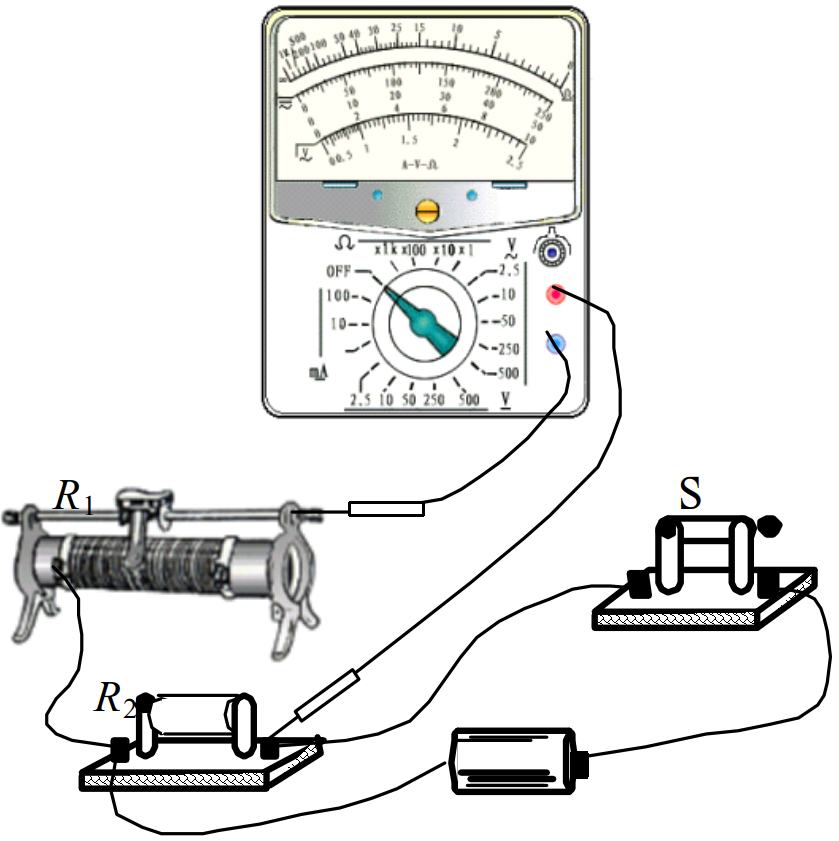
\includegraphics[width=0.5\linewidth]{picture/screenshot060}
\end{figure}

\begin{enumerate}
%\renewcommand{\labelenumi}{\arabic{enumi}.}
% A(\Alph) a(\alph) I(\Roman) i(\roman) 1(\arabic)
%设定全局标号series=example	%引用全局变量resume=example
%[topsep=-0.3em,parsep=-0.3em,itemsep=-0.3em,partopsep=-0.3em]
%可使用leftmargin调整列表环境左边的空白长度 [leftmargin=0em]
\item
若旋转选择开关,使其尖端对准直流电流档,此时测得的是通过 \underlinegap 的电流;

\item 
若断开电路中的电键,旋转选择开关使其尖端对准欧姆档,此时测得的是 \underlinegap 的阻值;

\item 
若旋转选择开关,使其尖端对准直流电压档,闭
合电键,并将滑动变阻器的滑片移至最左端,此时
测得的是 \underlinegap 两端的电压。

\end{enumerate}


\item 
(单选)在使用多用表的欧姆档测量电阻时,若 \underlinegap 。


\fourchoices
{双手捏住两表笔金属杆,测量值将偏大}
{测量时发现指针偏离中央刻度过大,则必需减小倍率,重新调零后再进行测量}
{选择“$ \times 10 $”倍率测量时发现指针位于 $ 20 $ 与 $ 30 $正中间,则测量值小于 $ 25 \ \Omega $}
{欧姆表内的电池使用时间太长,虽能完成调零,但测量值将略偏大}


\end{enumerate}

\tk{
\begin{enumerate}
%\renewcommand{\labelenumi}{\arabic{enumi}.}
% A(\Alph) a(\alph) I(\Roman) i(\roman) 1(\arabic)
%设定全局标号series=example	%引用全局变量resume=example
%[topsep=-0.3em,parsep=-0.3em,itemsep=-0.3em,partopsep=-0.3em]
%可使用leftmargin调整列表环境左边的空白长度 [leftmargin=0em]
\item
$ R_{1} $ \quad $ R_{1} $ 和 $ R_{2} $ 串联 \quad $ R_{2} $(或电源)
\item 
D
\end{enumerate}
} 



\item
\exwhere{$ 2015 $ 年上海卷}
如图是一个多用表欧姆档内部电路示意图。电流表满偏电流 $ 0.5 \ mA $、
内阻 $ 10 \ \Omega $;电池电动势 $ 1.5 \ V $、内阻 $ 1 \ \Omega $;变阻器 $ R_{0} $ 阻值 $ 0-5000 \ \Omega $。
\begin{figure}[h!]
\centering
\includesvg[width=0.23\linewidth]{picture/svg/GZ-3-tiyou-1019}
\end{figure}

\begin{enumerate}
%\renewcommand{\labelenumi}{\arabic{enumi}.}
% A(\Alph) a(\alph) I(\Roman) i(\roman) 1(\arabic)
%设定全局标号series=example	%引用全局变量resume=example
%[topsep=-0.3em,parsep=-0.3em,itemsep=-0.3em,partopsep=-0.3em]
%可使用leftmargin调整列表环境左边的空白长度 [leftmargin=0em]
\item
该欧姆表的刻度值是按电池电动势为 $ 1.5 \ V $ 刻度的,当电池的电
动势下降到 $ 1.45 \ V $、内阻增大到 $ 4 \ \Omega $时仍可调零。调零后 $ R_{0} $ 阻值将变 \underlinegap 
(选填“大”或“小”);若测得某电阻阻值为 $ 300 \ \Omega $,则这个电
\underlinegap 
阻的真实值是$ \Omega $。

\item 
若该欧姆表换了一个电动势为 $ 1.5 \ V $,内阻为 $ 10 \ \Omega $的电池,调零
后测量某电阻的阻值,其测量结果 \underlinegap (选填“偏大”、“偏小”或“准确”)。


\end{enumerate}

\tk{
\begin{enumerate}
%\renewcommand{\labelenumi}{\arabic{enumi}.}
% A(\Alph) a(\alph) I(\Roman) i(\roman) 1(\arabic)
%设定全局标号series=example	%引用全局变量resume=example
%[topsep=-0.3em,parsep=-0.3em,itemsep=-0.3em,partopsep=-0.3em]
%可使用leftmargin调整列表环境左边的空白长度 [leftmargin=0em]
\item
小 \quad $ 290 $
\item 
准确
\end{enumerate}
} 


\item 
\exwhere{$ 2011 $ 年理综安徽卷}
\item 
\begin{enumerate}
%\renewcommand{\labelenumi}{\arabic{enumi}.}
% A(\Alph) a(\alph) I(\Roman) i(\roman) 1(\arabic)
%设定全局标号series=example	%引用全局变量resume=example
%[topsep=-0.3em,parsep=-0.3em,itemsep=-0.3em,partopsep=-0.3em]
%可使用leftmargin调整列表环境左边的空白长度 [leftmargin=0em]
\item
某同学使用多用电表粗略测量一定值电阻的阻值,先把选择开关旋到“$ \times 1k $”挡位,测量时
指针偏转如图$ (a) $所示。请你简述接下来的测量过程:

① \hthreefullline[;] 

② \hthreefullline[;] 

③ \hthreefullline[;] 

④测量结束后,将选择开关旋到“$ OFF $”挡。


\item 
接下来采用“伏安法”较准确地测量该电阻的阻值,所用实验器材如图$ (b) $所示。其中电压表内阻约
为 $ 5 \ k\Omega $,电流表内阻约为 $ 5 \ \Omega $。图中部分电路已经连接好,请完成实验电路的连接。


\item 
图($ c $)是一个多量程多用电表的简化电路图,测量电流、电压和电阻各有两个量程。当转换开
关 $ S $ 旋到位置 $ 3 $ 时,可用来测量 \underlinegap 
;当 $ S $ 旋到位置
\underlinegap 
时,可用来测量电流,其中 $ S $
旋到位置 \underlinegap 时量程较大。


\end{enumerate}
\begin{figure}[h!]
\centering
\begin{subfigure}{0.4\linewidth}
\centering
\includesvg[width=0.7\linewidth]{picture/svg/GZ-3-tiyou-1021} 
\caption{}\label{}
\end{subfigure}
\begin{subfigure}{0.4\linewidth}
\centering
\includesvg[width=0.7\linewidth]{picture/svg/GZ-3-tiyou-1022} 
\caption{}\label{}
\end{subfigure}
\begin{subfigure}{0.4\linewidth}
\centering
\includesvg[width=0.7\linewidth]{picture/svg/GZ-3-tiyou-1023} 
\caption{}\label{}
\end{subfigure}
\end{figure}


\tk{
\begin{enumerate}
%\renewcommand{\labelenumi}{\arabic{enumi}.}
% A(\Alph) a(\alph) I(\Roman) i(\roman) 1(\arabic)
%设定全局标号series=example	%引用全局变量resume=example
%[topsep=-0.3em,parsep=-0.3em,itemsep=-0.3em,partopsep=-0.3em]
%可使用leftmargin调整列表环境左边的空白长度 [leftmargin=0em]
\item
①断开待测电阻,将选择开关旋到“$ \times 10^{0} $”档;\\
②将两表笔短接,调整“欧姆调零旋钮”,使指针指向“$ 0 \ \Omega $”; 
\\
③再接入待测电阻,将指针示数$ \times 100 $,即为待测电阻阻值。
\item 
如图所示
\begin{center}
\includesvg[width=0.23\linewidth]{picture/svg/GZ-3-tiyou-1024} 
\end{center}
\item 
电阻 \qquad 1、2 \qquad 1
\end{enumerate}
} 


\item
\exwhere{$ 2011 $ 年理综全国卷}
使用多用电表测量电阻时,多用电表内部的电路可以等效为一个直流电源(一般为电
池)
、一个电阻和一表头相串联,两个表笔分别位于此串联电路的两端。现需要测量多用电表内电
池的电动势,给定的器材有:待测多用电表,量程为 $ 60 \ mA $ 的
电流表,电阻箱,导线若干。实验时,将多用电表调至$ \times 1 \ \Omega $挡,
调好零点;电阻箱置于适当数值。完成下列填空:
\begin{enumerate}
%\renewcommand{\labelenumi}{\arabic{enumi}.}
% A(\Alph) a(\alph) I(\Roman) i(\roman) 1(\arabic)
%设定全局标号series=example	%引用全局变量resume=example
%[topsep=-0.3em,parsep=-0.3em,itemsep=-0.3em,partopsep=-0.3em]
%可使用leftmargin调整列表环境左边的空白长度 [leftmargin=0em]
\item
仪器连线如图 $ 1 $ 所示($ a $ 和 $ b $ 是多用电表的两个表笔)。若两
电表均正常工作,则表笔 $ a $ 为 \underlinegap (填“红”或“黑”)色;
\begin{figure}[h!]
\centering
\includesvg[width=0.23\linewidth]{picture/svg/GZ-3-tiyou-1025}
\end{figure}

\item 
若适当调节电阻箱后,图 $ 1 $ 中多用电表、电流表与电阻箱的示数分别如图 $ 2(a) $,$ (b) $,$ (c) $所示,则
多用电表的读数为 \underlinegap $ \Omega $,电流表的读数为 \underlinegap $ mA $,电阻箱的读数为 \underlinegap $ \Omega $;
\begin{figure}[h!]
\centering
\begin{subfigure}{0.4\linewidth}
\centering
\includesvg[width=0.7\linewidth]{picture/svg/GZ-3-tiyou-1026} 
\caption{}\label{}
\end{subfigure}
\begin{subfigure}{0.4\linewidth}
\centering
\includesvg[width=0.7\linewidth]{picture/svg/GZ-3-tiyou-1027} 
\caption{}\label{}
\end{subfigure}
\begin{subfigure}{0.4\linewidth}
\centering
\includesvg[width=0.7\linewidth]{picture/svg/GZ-3-tiyou-1028} 
\caption{}\label{}
\end{subfigure}

\end{figure}


\item 
将图 $ 1 $ 中多用电表的两表笔短接,此时流过多用电表的电流为 \underlinegap $ mA $;(保留 $ 3 $ 位有效数字)


\item 
计算得到多用电表内电池的电动势为 \underlinegap $ V $。(保留 $ 3 $ 位有效数字)


\end{enumerate}

\tk{
\begin{enumerate}
%\renewcommand{\labelenumi}{\arabic{enumi}.}
% A(\Alph) a(\alph) I(\Roman) i(\roman) 1(\arabic)
%设定全局标号series=example	%引用全局变量resume=example
%[topsep=-0.3em,parsep=-0.3em,itemsep=-0.3em,partopsep=-0.3em]
%可使用leftmargin调整列表环境左边的空白长度 [leftmargin=0em]
\item
黑
\item 
$ 14.0 \quad 53.0 \quad 4.6 $
\item 
$ 102 $
\item 
$ 1.54 $
\end{enumerate}
} 



\item 
\exwhere{$ 2016 $ 年上海卷}
在“用多用电表测电阻、电流和电压”的实验中:
\begin{enumerate}
%\renewcommand{\labelenumi}{\arabic{enumi}.}
% A(\Alph) a(\alph) I(\Roman) i(\roman) 1(\arabic)
%设定全局标号series=example	%引用全局变量resume=example
%[topsep=-0.3em,parsep=-0.3em,itemsep=-0.3em,partopsep=-0.3em]
%可使用leftmargin调整列表环境左边的空白长度 [leftmargin=0em]
\item
(多选题)用多用电测电流或电阻的过程中 \underlinegap .
\fourchoices
{在测量电阻时,更换倍率后必须重新进行调零}
{在测量电流时,更换量程后必须重新进行调零}
{在测量未知电阻时,必须先选择倍率最大挡进行试测}
{在测量未知电流时,必须先选择电流最大量程进行试测}




\item 
测量时多用电表指针指在如图所示位
置。若选择开关处于“$ 10 \ V $”挡,其读数为 \underlinegap $ V $;若选择开关处于“$ \times 10 $”挡,其读数为 \underlinegap 
$ 200 \ \Omega $(选填:“大于”,“等于”或“小于”)。
\begin{figure}[h!]
\centering
\includesvg[width=0.23\linewidth]{picture/svg/GZ-3-tiyou-1029}
\end{figure}

\end{enumerate}

\tk{
\begin{enumerate}
%\renewcommand{\labelenumi}{\arabic{enumi}.}
% A(\Alph) a(\alph) I(\Roman) i(\roman) 1(\arabic)
%设定全局标号series=example	%引用全局变量resume=example
%[topsep=-0.3em,parsep=-0.3em,itemsep=-0.3em,partopsep=-0.3em]
%可使用leftmargin调整列表环境左边的空白长度 [leftmargin=0em]
\item
$ 5.4 $
\item 
小于
\end{enumerate}
} 


\item 
\exwhere{$ 2018 $年浙江卷($ 4 $月选考)}
\begin{enumerate}
%\renewcommand{\labelenumi}{\arabic{enumi}.}
% A(\Alph) a(\alph) I(\Roman) i(\roman) 1(\arabic)
%设定全局标号series=example	%引用全局变量resume=example
%[topsep=-0.3em,parsep=-0.3em,itemsep=-0.3em,partopsep=-0.3em]
%可使用leftmargin调整列表环境左边的空白长度 [leftmargin=0em]
\item
小明用多用电表测量一小段$ 2B $铅笔芯的电阻$ R $,正
确的操作顺序是 \underlinegap (填字母);
\fivechoices
{把选择开关旋转到交流电压最高档}
{调节欧姆调零旋钮使指针指到欧姆零点}
{把红、黑表笔分别接在$ R_{x} $两端,然后读数}
{把选择开关旋转到合适的档位,将红、黑表笔接触}
{把红、黑表笔分别插入多用电表“$ + $”、“$ - $”插孔,用螺丝刀调节指针定位螺丝,使指针指$ 0 $}

\item 
小明正确操作后,多用电表的指针位置如图所示,则
$ R_{x} =$ \underlinegap $ \Omega $。
% TODO: \usepackage{graphicx} required
\begin{figure}[h!]
\centering
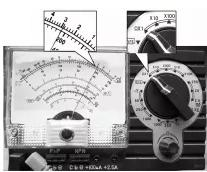
\includegraphics[width=0.47\linewidth]{picture/screenshot061}
\end{figure}

\item 
小张认为用多用电表测量小电阻误差太大,采用伏安法测量。

现有实验器材如下:电源(电动势$ 3 \ V $,内阻可忽略),电压表(量程$ 3 \ V $,内阻约为$ 3 \ k\Omega $),多用电
表($ 2.5 \ mA $挡、$ 25 \ mA $挡和$ 250 \ mA $挡,对应的内电阻约为$ 40 \ \Omega ,4 \ \Omega $和$ 0.4 \ \Omega $),滑动变阻器$ R_p $($ 0 \sim 10 \ \Omega $),
定值电阻$ R_{0} $(阻值$ 10 \ \Omega $),开关及导线若干。

测量铅笔芯的电阻$ R_{x} $,下列电路图中最合适的是 \underlinegap (填字母),多用电表选择开关应置于 \underlinegap 
挡。
\pfourchoices
{\includesvg[width=4.3cm]{picture/svg/GZ-3-tiyou-1030}}
{\includesvg[width=4.3cm]{picture/svg/GZ-3-tiyou-1031}}
{\includesvg[width=4.3cm]{picture/svg/GZ-3-tiyou-1032}}
{\includesvg[width=4.3cm]{picture/svg/GZ-3-tiyou-1033}}


\end{enumerate}

\tk{
\begin{enumerate}
%\renewcommand{\labelenumi}{\arabic{enumi}.}
% A(\Alph) a(\alph) I(\Roman) i(\roman) 1(\arabic)
%设定全局标号series=example	%引用全局变量resume=example
%[topsep=-0.3em,parsep=-0.3em,itemsep=-0.3em,partopsep=-0.3em]
%可使用leftmargin调整列表环境左边的空白长度 [leftmargin=0em]
\item
EDBCA
\item 
$ 2.8 \sim 3.0 $
\item 
B \quad $ 250 \ mA $
\end{enumerate}
} 






\item
\exwhere{$ 2017 $ 年新课标 \lmd{3} 卷}
图($ a $)为某同学组装完成的简易多用电表的电路图。图中 $ E $ 是电池;$ R_{1} $、$ R_{2} $、$ R_{3} $、$ R_{4} $ 和 $ R_{5} $ 是固定
电阻,$ R_{6} $ 是可变电阻;表头$ G $ 的满偏电流为 $ 250 \ \mu A $,内阻为 $ 480 \ \Omega $。虚线方框内为换挡开关,$ A $
端和 $ B $ 端分别于两表笔相连。该多用电表有 $ 5 $ 个挡位,$ 5 $ 个挡位为:直流电压 $ 1 \ V $ 挡和 $ 5 \ V $ 挡,直
流电流 $ 1 \ mA $ 挡和 $ 2.5 \ mA $ 挡,欧姆$ \times 100 \ \Omega $挡。
\begin{figure}[h!]
\centering
\begin{subfigure}{0.4\linewidth}
\centering
\includesvg[width=0.88\linewidth]{picture/svg/GZ-3-tiyou-1034} 
\caption{}\label{}
\end{subfigure}
\begin{subfigure}{0.4\linewidth}
\centering
\includesvg[width=0.88\linewidth]{picture/svg/GZ-3-tiyou-1035} 
\caption{}\label{}
\end{subfigure}
\end{figure}



\begin{enumerate}
%\renewcommand{\labelenumi}{\arabic{enumi}.}
% A(\Alph) a(\alph) I(\Roman) i(\roman) 1(\arabic)
%设定全局标号series=example	%引用全局变量resume=example
%[topsep=-0.3em,parsep=-0.3em,itemsep=-0.3em,partopsep=-0.3em]
%可使用leftmargin调整列表环境左边的空白长度 [leftmargin=0em]
\item
图($ a $)中的 $ A $ 端与 \underlinegap (填“红”或“黑”)色表笔相连接。


\item 
关于 $ R_{6} $ 的使用,下列说法正确的是 \underlinegap (填正确答案标号)。
\threechoices
{在使用多用电表之前,调整 $ R_{6} $ 使电表指针指在表盘左端电流“$ 0 $”位置}
{使用欧姆挡时,先将两表笔短接,调整 $ R_{6} $ 使电表指针指在表盘右端电阻“$ 0 $”位置}
{使用电流挡时,调整 $ R_{6} $ 使电表指针尽可能指在表盘右端电流最大位置}

\item 
根据题给条件可得 $ R_{1} + R_{2} =$ \underlinegap $ \Omega $,$ R_{4} = $ \underlinegap $ \Omega $。


\item 
某次测量时该多用电表指针位置如图($ b $)所示。若此时 $ B $ 端是与“$ 1 $”连接的,则多用电表读
数为 \underlinegap ;若此时 $ B $ 端是与“$ 3 $”连接的,则读数为 \underlinegap ;若此时 $ B $ 端是与“$ 5 $”连
接的,则读数为 \underlinegap 。
(结果均保留 $ 3 $ 为有效数字)



\end{enumerate}

\tk{
\begin{enumerate}
%\renewcommand{\labelenumi}{\arabic{enumi}.}
% A(\Alph) a(\alph) I(\Roman) i(\roman) 1(\arabic)
%设定全局标号series=example	%引用全局变量resume=example
%[topsep=-0.3em,parsep=-0.3em,itemsep=-0.3em,partopsep=-0.3em]
%可使用leftmargin调整列表环境左边的空白长度 [leftmargin=0em]
\item
黑
\item 
B
\item 
$ 160 \ \Omega \quad 880 \ \Omega $
\item 
$ 1.49 \ mA $;$ 11.0 \times 10^{0} \ \Omega $;$ 2.95 \ V $
\end{enumerate}
} 








\end{enumerate}

